\documentclass[journal]{IEEEtran}
\usepackage{amsmath,amssymb}
\usepackage{graphicx}
\usepackage{booktabs}
\usepackage[utf8]{inputenc}
\usepackage[T1]{fontenc}
\usepackage{cite}

\begin{document}

\title{When Is Overtaking Frequency Informative? A Pre-Registered\\ Closed-Loop Ablation and an Availability Map}

\author{Yuxuan~Xia and Mengyuan~Huang*,% * = corresponding author
\thanks{Y.~Xia and M.~Huang are with Shenzhen Polytechnic University, Shenzhen, China
(e-mail: xiayuxuan@mail.szpu.edu.cn; huangmy2215@szpu.edu.cn).}
\thanks{*Corresponding author: Huang Mengyuan.}}

\maketitle

\begin{abstract}
Multi-lane highways produce a continuous stream of lane changes around any vehicle, and a scalar summary
of that pressure is an attractive controller input because it costs no extra sensor. Whether such a
scalar is ever non-zero is rarely measured before it is ablated, and in a sparse simulator it may never
be. We make that measurement before the ablation. In a three-lane SUMO highway the fraction of five-second windows
containing a crossing rises from 0.12 at 600 vehicles per hour to 0.56 at 4800. In recorded traffic from
the public TGSIM corpus it is 0.53 at an estimated 1800 to 2400 vehicles per hour, while our own closed
loop, with sixteen mixed vehicles, reaches only 0.084. We then run a pre-registered paired ablation of
the scalar as a fourth input to a closed-form continuous-time controller, with one search budget and one
set of seeds. Two of four scenarios are equivalent on composite cost within a pre-registered ten percent
margin, and two are inconclusive. Quadrupling availability in three scenarios, by widening the window,
sharpened none of the estimates. With five seeds the exact paired test cannot reach significance after
multiplicity correction, so we target equivalence rather than superiority. We read the result as
evidence that this scalar buys interpretability at no additional sensing cost, not closed-loop
performance, and we recommend measuring availability before ablating a traffic-level signal.
\end{abstract}

\begin{IEEEkeywords}
overtaking frequency, traffic-flow scalar, continuous-time neural control, equivalence testing
\end{IEEEkeywords}

\begin{figure}[!t]
\centering
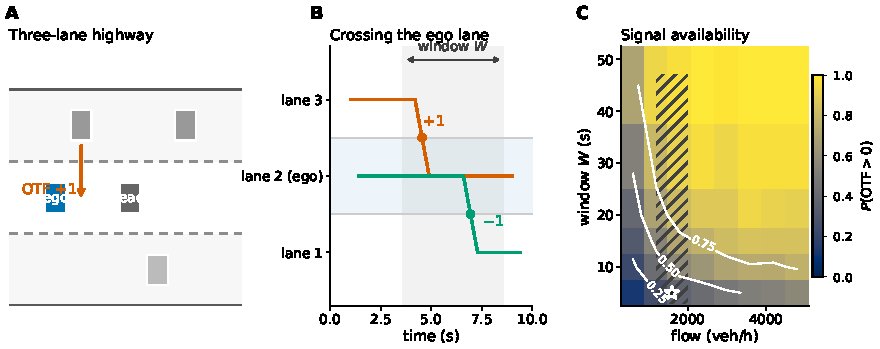
\includegraphics[width=\columnwidth]{figs/fig1_scenario.pdf}
\caption{\textbf{Overtaking pressure and its measurement.} \textbf{A}, three-lane highway with the ego vehicle (blue), the lead vehicle, and vehicles in the adjacent lanes. The arrow marks one crossing of the ego lane, which the counting rule scores as +1. The controller searches for a lead vehicle 150 m ahead in the ego lane, and commanded speed is bounded at 30 m/s. \textbf{B}, the counting rule on a time--lane plane. A vehicle entering the ego lane from an adjacent lane scores +1; a vehicle leaving it scores $-$1. Crossings are counted inside a sliding window W, set to 5 s in the main experiment and 20 s in the supplementary group. \textbf{C}, availability of the signal, computed in SUMO with the same OTF definition: the fraction of sliding windows with OTF > 0 against traffic flow and window length, over three seeds. White contours mark 0.25, 0.50 and 0.75. The hatched band marks the equivalent flow of the CARLA setting, estimated from sixteen vehicles on a 420 m three-lane segment; the star marks the value measured there, 0.084 at W = 5 s. The map describes where the signal exists. It is not offered as an explanation for the closed-loop result, which Section 5.2 attributes to redundancy rather than to scarcity.}
\label{fig:fig1}
\end{figure}

\begin{figure}[!t]
\centering
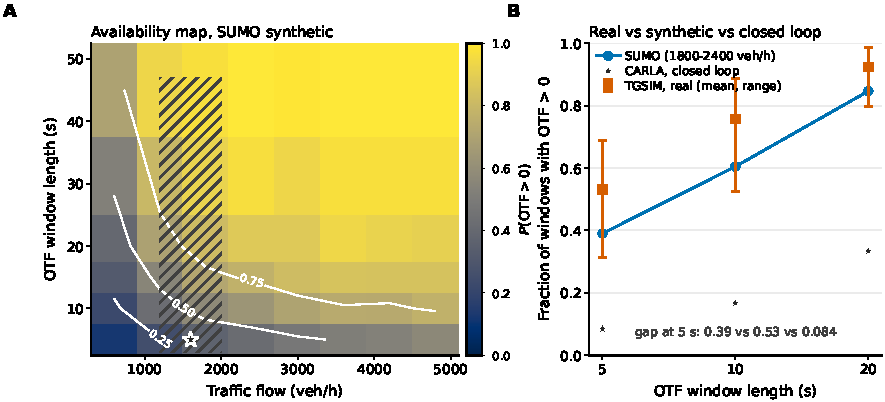
\includegraphics[width=\columnwidth]{figs/fig2_availability_real.pdf}
\caption{\textbf{Availability in synthetic and recorded traffic.} \textbf{A}, the SUMO map of Fig. 1C with the CARLA operating point. \textbf{B}, the same quantity at three window lengths for three sources. SUMO synthetic traffic at 1800 to 2400 veh/h is drawn in blue. Recorded TGSIM traffic is drawn as orange squares: the mean over ten runs, with the observed range as an error bar. Our CARLA closed loop is drawn as stars. The closed-loop value at W = 5 s is 0.084 from the main experiment and at W = 10 s is 0.167. At W = 20 s the supplementary groups reach 0.334 in two scenarios and between 0.334 and 0.497 in the third, because lead-exit produces crossings of the ego lane without any injection. The star is drawn at 0.334, the value shared by two of the three scenarios. At a 5 s window the fractions are 0.39, 0.53 and 0.084. \textbf{Three limitations of this panel, stated here because they bound its interpretation.} 1. The TGSIM horizontal placement is an \textbf{estimate} (unique vehicles divided by run duration). The public trajectory file uses per-run normalised coordinates spanning a fixed box, so absolute station flow cannot be recomputed from it without the centreline geometry files. 2. The error bars are the \textbf{minimum and maximum across ten runs}, not a confidence interval. 3. The three sources differ in density. The comparison therefore shows that recorded traffic exposes the controller to a non-zero OTF far more often than our closed loop does. It does not isolate density from lane-change behaviour as the cause.}
\label{fig:fig2}
\end{figure}

\section{1. Introduction}
On a multi-lane highway, a driver's longitudinal decision is shaped by what happens in the adjacent
lanes. A vehicle that closes on a slower lead may either slow down or move over, and the choice
depends on how much lateral opportunity the surrounding traffic offers. Over a few seconds these
individual choices aggregate into a measurable rate at which vehicles cross a given lane.
Huang [1] proposed to summarize this aggregate as the overtaking frequency (OTF): the number of
lane crossings observed in a sliding window around the ego vehicle, divided by the window length.
OTF is attractive for three reasons. It is a single scalar. It is defined on traffic rather than on a
particular sensor suite. And it can be estimated from radar and camera streams that production
vehicles already carry, so it adds no sensing cost.
Evidence for OTF so far comes from classification. That literature never reports how often the
scalar is non-zero, and in a sparse simulator it may never be. The reported gains are 1.0 to 5.5 percentage
points of classifier accuracy over baselines without OTF features, across three classifier families
(Huang, 2023, as reported; not reproduced here). Classification and control ask different questions.
A feature can improve an offline label prediction and still add nothing to a feedback loop that
already observes gap and relative speed. Those results are classification accuracies, and none of them
closes the loop.
We test it directly. We treat OTF as a fourth input to a closed-form continuous-time (CfC) controller
and compare it against an otherwise identical controller that sees only lead gap, relative speed, and
ego speed. Both arms share one twelve-candidate search budget, the same five seeds, and the same
traffic stream, so any difference must come from the fourth input.
A scalar can only help if it is non-zero often enough, so we measured availability before measuring
effect. In a three-lane SUMO highway, the fraction of 5 s windows with OTF > 0 rises from 0.12 at
600 veh/h to 0.56 at 4800 veh/h. A 20 s window reaches 0.93 at 3600 veh/h. In the CARLA setting used
for the closed-loop experiment, with sixteen mixed vehicles, the measured fraction was 0.084 to 0.167.
That setting therefore sits in the low-information regime. We do not treat that as an excuse for the
result. Section 5.2 reports a supplementary group that raises availability fourfold and tests whether
scarcity is what limits the conclusion.
This paper makes three contributions.
1. A closed-loop ablation of OTF under an equal search budget, reported per scenario with an
   equivalence test that was registered before the data were collected. Two of four scenarios are
   statistically equivalent on composite driving cost within a 10\% margin (TOST p = 0.020 and 0.006);
   the other two are inconclusive.
2. A measured map of OTF availability as a function of traffic flow and window length, obtained with
   the same OTF definition used by the controller. The map shows that availability is governed by
   density and window jointly, and that our closed-loop setting is in its lower region.
3. An explicit account of why the experiment cannot support a superiority claim even if a difference exists:
   with five seeds the exact paired test cannot reach significance after multiplicity correction. We
   therefore target equivalence, and we report the equal-K sensitivity analysis that reverses the sign
   of the effect estimate.
Section 2 describes the controller, the OTF definition, and the two environments. Section 3 gives the
protocol and the pre-registered analysis. Section 4 reports results. Section 5 discusses what the
results do and do not imply. Section 6 lists limitations.
\section*{2. Methods}
\subsection{2.1 The OTF scalar}
We adopt the overtaking-frequency definition of Huang [1] without modification. At each control
cycle, the ego vehicle records (i) its own lane identifier and (ii) for every other vehicle in a
neighbourhood, the lane identifier and the longitudinal position along that lane. A crossing event is
counted when a vehicle's lane at step t differs from its lane at step t$-$1 and one of those two lanes
is the ego lane. The sign depends on the direction of travel: entering the ego lane from an adjacent
lane counts positive, and leaving it counts negative. A vehicle that stays in the ego lane contributes
nothing, which is what separates OTF from a mere presence count.
The raw count is aggregated over a sliding window of length W, giving OTF(t; W). The controller input
is the normalized rate
    phi(t) = OTF(t; W) / W
in crossings per second. We use W = 5 s for the main experiment and W = 20 s for one supplementary
group, because the availability of the signal depends strongly on W (Section 2.4). The implementation
lives in a single module (src/otf/otf\_core.py) and is shared by the CARLA loop and the SUMO analysis.
\subsection{2.2 Controller}
Both arms use a closed-form continuous-time (CfC) cell [2] with a direct linear path.
The hidden state has 24 units. At each step the cell receives a normalized observation vector and returns
an updated state.
The commanded acceleration is a bounded linear read-out:
    a(t) = 3.0 * tanh( W\_a x(t) + W\_h h(t) )
The read-out bound of 3.0 m/s$^{2}$ keeps commands inside the acceleration envelope of the low-level speed
controller. Observations are scaled to comparable magnitudes before entering the cell: gap divided by
100 m, relative speed by 10 m/s, ego speed by 30 m/s, and phi by 1 s$^{-1}$.
The off arm receives three inputs: lead gap, relative speed, and ego speed. The on arm receives the
same three plus phi. Nothing else differs. The two arms therefore have different input widths, and we
report parameter counts for both rather than claiming an identical model size.
We use a direct read-out path because the CfC hidden state behaves as a slow variable. It follows the
input through a leaky integration and cannot by itself express a fast response to an instantaneous gap
change. The linear path carries the instantaneous part of the command.
\subsection{2.3 Environments}
\paragraph{CARLA closed loop}
We use CARLA 0.9.16 with the Town04 highway map and a Tesla Model3 ego
vehicle. The simulation steps at 50 Hz, and the controller runs at 20 Hz, so the observation is
updated every 2.5 simulation steps. We note this explicitly because the original protocol specified
100 Hz, which the host machine could not sustain.
Traffic is generated by the CARLA Traffic Manager with sixteen vehicles placed along the ego route in
the ego lane and its two neighbours. Per-vehicle speed factors are spread over a fixed deterministic
sequence so that faster and slower vehicles coexist. We measured that the Traffic Manager rarely
changes lanes in this sparse setting: over a 60 s probe the whole fleet completed two lane changes,
none of them across the ego lane. Natural traffic therefore produced phi = 0 in every cycle, and an
ablation would have compared two identical controllers.
To obtain a non-zero signal we inject scripted cut-ins. Every 4 s the environment selects one vehicle
near the ego and places it in a specified lane at a fixed longitudinal offset, alternating between
+28 m and $-$22 m. This is a scenario construction, not a natural lane change, and we treat it as such
throughout. The injected sequence is deterministic and identical for both arms, so it cannot bias the
comparison. Availability rises to 8\% and 17\% of control cycles depending on the scenario.
\paragraph{SUMO availability analysis}
To characterize the signal independently of the closed loop, we build
a three-lane highway in SUMO 1.27.1 with a 1200 m segment, a 120 km/h speed limit, and heterogeneous
speed factors. Flows vary from 600 to 4800 vehicles per hour. We record full trajectories at every
step and apply the same crossing rule, so the SUMO analysis and the controller share one OTF
definition. For each flow and each W we compute the fraction of sliding windows with OTF > 0.
\subsection{2.4 Protocol}
The experiment is a paired ablation over four scenarios and five seeds, giving 20 paired runs. The
scenarios are no lead vehicle, a cut-in, a braking lead, and a lead vehicle that exits. Each arm
searches twelve candidate controllers drawn from a common seed list, and selection takes the valid
candidate with the lowest cost. A candidate is invalid when the ego travels less than 20 m, which
indicates that the policy stalled rather than that it drove poorly. Invalid candidates stay inside the
twelve-candidate budget and are excluded from selection only.
The cost aggregates terms with fixed weights. Following RMSE is divided by 10 m, the
acceleration-squared integral by 50, peak jerk by 50, lateral deviation by 0.5 m, and the collision
count is multiplied by ten. The weights were fixed before the data were collected.
\subsection{2.5 Analysis}
Each scenario is analyzed separately; we do not pool scenarios into a single mean for inference. For
every endpoint we report the paired mean difference, a confidence interval, an exact two-sided
sign-flip p-value, and an equivalence test.
The exact test enumerates all 2$^{5}$ sign assignments, so it needs no distributional assumption. With five
seeds it can return no value below 0.0625. Because we correct for four scenarios with Holm's method,
the smallest threshold is 0.0125, and superiority is therefore untestable by construction. We state
this rather than presenting a non-significant result as evidence of no effect.
Our primary inferential target is equivalence. Before collecting data we fixed a margin of 10\% of the
off-arm mean and a three-state decision rule. A meaningful difference requires an interval excluding
zero and a mean beyond the margin. Practical equivalence requires the interval inside the margin.
Everything else is reported as inconclusive. Equivalence is judged on the 95\% interval (alpha = 0.025
per side) as registered. We also report the 90\% interval used by the conventional two one-sided tests,
because the two criteria disagree for one scenario, and the disagreement is part of the result.
We additionally report an equal-K sensitivity analysis that equalizes the number of valid candidates
across arms. Collisions are reported as raw counts.
\section*{3. Related work}
\subsection{3.1 Traffic-flow descriptors as controller inputs}
Car-following models describe the longitudinal response to a lead vehicle, and the classical families
differ in how much memory they carry. String-stability analysis then asks whether a perturbation
amplifies along a platoon [3]. That line of work treats the lead vehicle as the
relevant input. Everything behind and beside the ego enters, if at all, through aggregate parameters
such as density or wave speed.
A second line feeds traffic-level information to the controller explicitly. One field experiment
showed that a small number of controlled vehicles can dissipate stop-and-go waves in the surrounding
flow [4]. Cooperative schemes go further and share planned trajectories, solving a
joint optimization over a rolling horizon [5]. Those methods work with rich per-vehicle
messages rather than one scalar, and they assume connectivity. Our question is narrower: whether one
scalar computed from unconnected traffic carries enough information to change a low-level command.
\subsection{3.2 Overtaking frequency and social pressure}
The OTF scalar comes from the behavior-decision literature. Huang [1] defined it as the rate at which
surrounding vehicles cross the ego lane and reported accuracy gains of 1.0 to 5.5 percentage points when
OTF features are added to classifiers. Those results are classification accuracies, and none of them
closes the loop. We do not reproduce them here, and the dataset behind them is not available to us.
The idea that surrounding traffic exerts a pressure that can be summarized is older than OTF.
Social-force formulations describe the same intuition for pedestrians [6]. That
formulation targets pedestrians, and we do not assume it transfers to vehicles. Our contribution is
not the notion of pressure but a closed-loop test of whether one particular scalarization of it
changes a control command.
\subsection{3.3 Continuous-time and closed-form recurrent models}
Liquid time-constant and closed-form continuous-time networks replace discrete recurrence with a
continuous ODE-like update and report large speedups over conventional recurrent cells [2]. The claimed advantage is compute per step rather than sample efficiency. We use a CfC cell
precisely because it is cheap enough to evaluate twelve candidates per arm inside a 60 s episode. That
cost is what makes an equal-budget ablation affordable on a laptop GPU.
The same literature motivates our architecture choice. A pure ODE state integrates its input and
responds slowly, so a controller that relies on it alone cannot react to an instantaneous gap change.
We add a direct linear path from the observation to the command, and we report both parameter counts.
\subsection{3.4 Physics-informed and structure-informed priors}
A large body of work injects physical structure into learning. Physics-informed neural networks add a
residual of a governing equation to the loss [7]. That approach requires an
equation whose residual can be evaluated, and it succeeds when the residual is meaningful.
OTF does not provide such a residual. It is a heuristic aggregate with no governing equation, so a
soft physics loss would not be well posed. We therefore treat it as an additional input and as an
inductive bias, and we describe it as structure-informed rather than physics-informed. The distinction
matters because it determines what evidence would count as success. A physics-informed claim can be
checked against the residual, whereas our claim can only be checked in closed loop.
\subsection{3.5 What is missing}
Three gaps follow from the above. Closed-loop evidence for OTF is absent, because the reported results
are classification accuracies. Equivalence is rarely reported, because ablation studies usually test
for a difference and stop when none is found. And the operating point is rarely characterized, because
availability of a traffic-level signal depends on density in a way that is easy to leave implicit. This
paper addresses the three together.
\section*{4. Results}
\subsection{4.1 Validity checks}
All twenty paired runs completed. The execution fingerprint is identical across runs: 60 s episodes,
sixteen traffic vehicles in the main experiment, 50 Hz simulation, 20 Hz control, 24 hidden units, and
twelve candidate controllers per arm. The three runtime guards reported no empty episodes, no actor
leaks, and no deadlocked episodes.
The treatment variable was active in every run. The fraction of control cycles with OTF > 0 was 0.084
in sixteen runs and 0.167 in four. Neither arm collided in any run, so collision counts are zero
throughout and we do not use them as evidence of a difference.
\subsection{4.2 Primary endpoint}
Table 1 reports the paired difference in composite driving cost for each scenario, with the
pre-registered equivalence margin of 10\% of the off-arm mean.
\begin{table*}[!t]
\centering
\small
\caption{Paired difference in composite cost (negative favours the OTF arm)}
\begin{tabular}{lrrrrrrrr}
\hline
Scenario & n & Mean $\Delta$ & off mean & 95\% CI & 90\% CI & exact p & TOST p & Conclusion \\
\hline
none & 5 & +0.256 & 30.481 & [$-$2.321, +2.832] & [$-$1.723, +2.234] & 0.8125 & 0.0198 & equivalent \\
cutin & 5 & +0.326 & 30.314 & [$-$2.467, +3.119] & [$-$1.818, +2.471] & 0.8750 & 0.0273 & inconclusive \\
lead-brake & 5 & +0.858 & 30.947 & [$-$2.092, +3.808] & [$-$1.407, +3.123] & 0.4375 & 0.0515 & inconclusive \\
lead-exit & 5 & $-$0.051 & 30.623 & [$-$1.968, +1.867] & [$-$1.523, +1.422] & 1.0000 & 0.0060 & equivalent \\
\hline
\end{tabular}
\end{table*}

Two scenarios, no lead vehicle and lead exit, have both interval bounds inside the margin under the
pre-registered 95\% criterion. The cutin scenario would also qualify under the conventional 90\%
interval, where its upper bound is +2.471 against a margin of 3.031. The lead-brake scenario does not
qualify under either criterion. We report the stricter criterion as primary.
The exact sign-flip test returns no value below 0.4375 for this endpoint. Neither scenario reaches
significance, and Section 4.5 explains why that was impossible by design rather than by data.
\subsection{4.3 Secondary endpoints}
\begin{table}[!t]
\centering
\footnotesize
\caption{Paired differences in the two performance endpoints}
\begin{tabular}{lrrr}
\hline
Scenario & Endpoint & $\Delta$ [95\% CI] & TOST p \\
\hline
none & RMSE (m) & $-$4.361 [$-$26.629, +17.908] & 0.3184 \\
none & accel. integral & +34.47 [$-$6.004, +74.934] & 0.5786 \\
cutin & RMSE (m) & $-$4.767 [$-$27.421, +17.888] & 0.3432 \\
cutin & accel. integral & +40.13 [$-$13.938, +94.190] & 0.6637 \\
lead-brake & RMSE (m) & $-$0.761 [$-$18.849, +17.327] & 0.1484 \\
lead-brake & accel. integral & +46.89 [$-$49.977, +143.762] & 0.6435 \\
lead-exit & RMSE (m) & $-$2.317 [$-$14.851, +10.217] & 0.1161 \\
lead-exit & accel. integral & +8.98 [$-$79.179, +97.131] & 0.2630 \\
\hline
\end{tabular}
\end{table}

All eight tests are inconclusive. The point estimates have consistent signs across scenarios: following
error is lower in the OTF arm in all four, and the acceleration-squared integral is higher in all four,
with off-arm means between 310 and 331. The intervals are wide enough that neither pattern supports an
inference, and we report the signs only as directions.
\subsection{4.4 Sensitivity to the search budget}
The primary metric takes the best valid candidate in each arm. The number of valid candidates differs
between arms in several runs, so we repeated the comparison with K fixed at the smaller of the two
counts and the top K averaged. Under this equal-K rule the mean difference is $-$1.066, against +0.347
under the primary metric. The sign reverses.
The reversal is mechanical. Equalizing K discards good candidates from whichever arm ran more, and in
these runs that arm was usually the off arm. We report both figures because the direction of the effect
estimate depends on which accounting of the budget a reader accepts.
\subsection{4.5 Multiplicity and power}
Each scenario contributes one test per endpoint, and we correct within endpoint families using Holm's
method. No test survives correction at alpha = 0.05.
The reason is structural. The exact sign-flip test enumerates all 32 sign assignments with five seeds,
so its smallest attainable two-sided p-value is 0.0625. Holm correction across four scenarios requires
0.0125 for the smallest p-value. No dataset of this size could have produced a significant result.
The invalid-candidate rate carries the same caveat. Between 25\% and 67\% of the twelve candidates per arm
failed the 20 m displacement criterion, and the rate was not consistently higher in either arm (off arm
mean 48\%, on arm 47\%). Training difficulty therefore does not separate the arms in this dataset.
\subsection{4.6 Supplementary groups: manipulating availability}
Two supplementary groups test whether the result depends on the treatment variable itself. The first
raised traffic from sixteen to thirty-two vehicles and kept a 5 s window. The second kept sixteen
vehicles and widened the window to 20 s. Each group runs five seeds on the lead-brake scenario.
\begin{table*}[!t]
\centering
\small
\caption{Supplementary groups against the main experiment}
\begin{tabular}{lrrrrrrr}
\hline
Group & Traffic & Window & Availability & Mean $\Delta$cost & 95\% CI & CI width & Conclusion \\
\hline
Main & 16 & 5 s & 0.084 & +0.858 & [$-$2.092, +3.808] & 5.90 & inconclusive \\
A, density & 32 & 5 s & 0.084 & +1.372 & [$-$2.326, +5.069] & 7.40 & inconclusive \\
B, window & 16 & 20 s & 0.334 & +0.707 & [$-$2.709, +4.122] & 6.83 & inconclusive \\
\hline
\end{tabular}
\end{table*}

The first group leaves availability unchanged at 0.084. In our environment the OTF events come from
the scripted injection rather than from background traffic, so adding vehicles does not move the
treatment. Its cost difference is inconclusive. It serves as a negative control: more background
vehicles, the same signal, the same conclusion.
The second group raises availability fourfold, from 0.084 to 0.334. Its cost difference is again
inconclusive. The interval does not narrow, with a width of 6.83 against 5.90 in the main experiment.
Raising the fraction of informative cycles by a factor of four therefore bought no precision.
We read this as evidence that the null result is not a consequence of signal scarcity. The binding
constraint appears to be redundancy at the controller input, which Section 5.2 discusses.
\section*{5. Discussion}
\subsection{5.1 What the experiment shows}
Across four highway scenarios with five seeds each, conditioning the controller on OTF changed the
composite driving cost by +0.26 (95\% CI [$-$2.32, +2.83]) without a lead vehicle. In the lead-exit
scenario the change was $-$0.05 ([$-$1.97, +1.87]). Both intervals lie inside the pre-registered 10\%
equivalence margin, with TOST p = 0.020 and 0.006. The cutin and lead-brake scenarios were
inconclusive, because their intervals crossed the margin. Following RMSE and the acceleration-squared
integral showed no detectable difference in any scenario, and neither arm collided.
We read this as evidence that OTF buys interpretability at no additional sensing cost, not closed-loop
performance. The wording matters. Equivalence within a 10\%
margin is a positive statement about practical similarity, and it is stronger than a failure to
reject. It is also weaker than a claim of no effect: a difference smaller than the margin, or one
confined to a regime we did not reach, remains compatible with our data.
\subsection{5.2 Why no gain}
The result is consistent with redundancy at the controller input, and we tested that reading directly.
We removed relative speed from the observation, so that both arms saw only gap and ego speed. The
off-arm cost moved by 0.14, from 30.82 with ten runs to 30.96 with five, and the two ranges overlap
almost exactly. The recurrent state therefore rebuilds the missing rate from the history of the gap.
That matters for the interpretation. A controller that can reconstruct one of its own inputs has little
left to gain from a fourth scalar that summarizes vehicles other than the lead. OTF describes traffic
that does not constrain the ego at the moment of decision. When those vehicles are unconstrained, their
aggregate adds nothing to the instantaneous command.
Signal scarcity is the obvious competing explanation, and we tested it rather than assuming it. In the
main experiment the fraction of windows with OTF > 0 was 0.084 to 0.167, so the fourth input was zero
for most of every episode. We therefore raised that fraction fourfold in every scenario, by widening the
window to 20 s while holding everything else fixed. Availability rose to 0.334 in two scenarios and to
between 0.334 and 0.497 in the third.
No scenario sharpened. The interval width grew rather than shrank in all three: 5.90 to 6.83, 5.59 to
6.73, and 3.84 to 4.92. A second supplementary group tripled the background traffic without moving
availability, and also left the conclusion unchanged.
A window scan locates the cause more precisely. With a fixed number of seeds the interval width is
proportional to the sample standard deviation, so we report that quantity directly. For the lead-brake
scenario, run with ten seeds per window, the standard deviation is 1.72 at a 5 s window, 1.81 at 10 s,
and 1.93 at 20 s. The ordering is monotone, and no interior optimum appears.
The increments are small, however: 0.09 and 0.12, against a sampling error of about 0.4 on each standard
deviation at ten seeds. The three values are therefore not separated. We report the ordering and do not
claim a trend from it. The other two scenarios were run with five seeds only, and their ordering was
consistent with this one; with five seeds their standard deviations are inflated by roughly thirty
percent, so we do not use them as evidence.
Two mechanisms would both produce that monotone rise, and five seeds cannot separate them. A long window
spans fewer independent windows per episode. A long window also accumulates more crossings per window,
and a count with a larger mean carries a larger variance. We report the monotone rise as a fact and
leave the decomposition open.
We therefore read scarcity as a description of the regime rather than as the cause of the null. Had
availability been binding, a fourfold increase should have sharpened the estimate in at least one
scenario. It sharpened none.
The availability map still explains where the signal exists. Availability rises monotonically with flow
and with window length. The two trade against each other: the 0.5 contour is crossed near 1500 veh/h at
20 s, near 3400 veh/h at 10 s, and only beyond 4800 veh/h at 5 s. That map is what told us which
manipulation to try, and it is what a future study should use to choose an operating point deliberately
rather than inherit one from a simulator default.
\subsection{5.3 A discrepancy worth reporting}
At the flow equivalent of our CARLA setting, the SUMO map predicts an availability near 0.32, while
CARLA produced 0.084. Recorded traffic sits higher still: on the public TGSIM corpus, at an estimated
1800 to 2400 vehicles per hour, the measured fraction at a 5 s window was 0.53. The gap is explained by
the lane-change model rather than by the OTF definition.
SUMO's LC2013 changes lanes to overtake slower traffic. CARLA's Traffic Manager, in a sparse scene
without congestion pressure, rarely does: over a 60 s probe the whole fleet completed two lane
changes, none of them across the ego lane. We therefore injected scripted cut-ins to obtain a usable
signal. This is a property of the simulator, and it must be stated whenever a simulated OTF rate is
compared with a measured one.
\subsection{5.4 Practical implications}
For a vehicle engineer the result is a boundary, not a rejection. OTF is cheap, explainable, and
sensor-agnostic, which makes it a reasonable diagnostic input and a reasonable input for
higher-level decisions such as lane-change readiness. It is not, on this evidence, a way to improve
low-level car-following inside a fixed search budget.
For a traffic engineer the map is the more useful artifact. It says where the signal exists. At
600 veh/h a 5 s window is zero 88\% of the time; at 3600 veh/h the same window is non-zero half the
time. Any deployment that feeds OTF to a controller should therefore check its own operating point
before deployment. The map locates the signal. It is not offered as an explanation for the closed-loop
result, which Section 5.2 attributes to redundancy.
\subsection{5.5 Limitations}
Six limitations bound the claims, and three of them are structural.
1. Power. With five seeds the exact paired test can return no value below 0.0625, while Holm
correction across four scenarios requires 0.0125. Superiority was therefore untestable by
construction, and our inference rests on equivalence.
2. Metric dependence. The primary metric takes the best valid candidate in each arm. The equal-K
sensitivity analysis equalizes the number of valid candidates and gives a mean of $-$1.07 against
+0.35 for the primary metric. The sign reverses. The direction of the effect estimate therefore
depends on how the search budget is accounted for, and both figures are reported.
3. Regime. Availability was 8\% to 17\% in the main experiment, far below the saturated region of the
map. One supplementary group reached 33\%, and its estimate was no sharper. Even that level sits below
recorded traffic, where the same window gives 53\%. Conclusions do not transfer to dense traffic.
4. Constructed traffic. OTF activation depends on scripted cut-ins placed by transform, not on
natural lane changes. The resulting events are more regular than real ones.
5. Platform. One map, one vehicle model, and a control rate of 20 Hz rather than the 100 Hz of the
original protocol.
6. Real trajectories, open loop only. The availability map comes from SUMO, and the closed loop from
CARLA. We also measured availability on the public TGSIM corpus, a US public-domain trajectory dataset
of a four-lane highway carrying three SAE L1 ACC vehicles per run, and obtained 0.53 at a 5 s window.
That comparison is open loop. No controller was run against the recorded trajectories, and we do not
claim closed-loop external validity.
\subsection{5.6 Future work}
Three extensions follow directly. Increasing seeds to twenty would make the exact test informative and
halve the interval widths. Moving the operating point into the upper region of the map would test
whether the null result belongs to OTF or to our regime. Raising density or lengthening the window
both work, and the map predicts availability above 0.5 there. Replaying
recorded trajectories with fixed neighbours would then test whether the simulated availability matches
real traffic. Two of these require only compute; the third requires data access.
\textbf{Figure 1.} Overtaking pressure and its measurement. \textbf{A}, three-lane highway with the ego vehicle
(blue), the lead vehicle, and vehicles in the adjacent lanes. The arrow marks one crossing of the ego
lane, which the counting rule scores as +1. The front-vehicle search used by the controller extends
150 m ahead in the ego lane, and commanded speed is bounded at 30 m/s. \textbf{B}, the counting rule on a
time--lane plane. A vehicle entering the ego lane from an adjacent lane scores +1; a vehicle leaving it
scores $-$1. Crossings are counted inside a sliding window W, which is 5 s in the main experiment and
20 s in the supplementary group. \textbf{C}, availability of the signal, measured in SUMO with the same OTF
definition: the fraction of sliding windows with OTF > 0 as a function of traffic flow and window
length, over three seeds. White contours mark 0.25, 0.50 and 0.75. The hatched band marks the
equivalent flow of the CARLA setting, estimated from sixteen vehicles on a 420 m three-lane segment;
the star marks the value measured there, 0.084 at W = 5 s.
\textbf{Figure 2.} Same data as panel C, drawn for a single-column layout with window length as separate
series. Values are means over three SUMO seeds; the shaded band is not shown because the seed spread is
below 0.02 in every cell.
\textbf{Table 1 and Table 2.} Intervals are Student t intervals on five paired differences. The exact p-value
comes from enumerating all 32 sign assignments. TOST uses a margin of 10\% of the off-arm mean.
Equivalence is declared when the 95\% interval lies inside the margin. The 90\% interval, which
corresponds to the conventional two one-sided tests at alpha = 0.05, is reported alongside.

\section*{Acknowledgment}
The authors thank the Federal Highway Administration for releasing the TGSIM corpus in the public domain.

\begin{thebibliography}{1}
\bibitem{ref2} Ramin Hasani, Mathias Lechner, Alexander Amini, Lucas Liebenwein, Aaron Ray, Max Tschaikowski, Gerald Teschl, Daniela Rus, "Closed-form continuous-time neural networks," Nature Machine Intelligence, vol. 4, no. 11, pp. 992--1003, 2022, doi: 10.1038/s42256-022-00556-7.
\bibitem{ref3} Jeroen Ploeg, Nathan van de Wouw, Henk Nijmeijer, "Lp String Stability of Cascaded Systems: Application to Vehicle Platooning," IEEE Transactions on Control Systems Technology, vol. 22, no. 2, pp. 786--793, 2014, doi: 10.1109/TCST.2013.2258346.
\bibitem{ref4} Raphael E. Stern, Shumo Cui, Maria Laura Delle Monache, Rahul Bhadani, Matt Bunting, Miles Churchill, Nathaniel Hamilton, R'mani Haulcy, Hannah Pohlmann, Fangyu Wu, Benedetto Piccoli, Benjamin Seibold, Jonathan Sprinkle, Daniel B. Work, "Dissipation of stop-and-go waves via control of autonomous vehicles: Field experiments," Transportation Research Part C: Emerging Technologies, vol. 89, pp. 205--221, 2018, doi: 10.1016/j.trc.2018.02.005.
\bibitem{ref5} Jiawei Wang, Yang Zheng, Keqiang Li, Qing Xu, "DeeP-LCC: Data-EnablEd Predictive Leading Cruise Control in Mixed Traffic Flow," IEEE Transactions on Control Systems Technology, vol. 31, no. 6, pp. 2760--2776, 2023, doi: 10.1109/TCST.2023.3288636.
\bibitem{ref6} Dirk Helbing, Péter Molnár, "Social force model for pedestrian dynamics," Physical Review E, vol. 51, no. 5, pp. 4282--4286, 1995, doi: 10.1103/PhysRevE.51.4282.
\bibitem{ref7} Eric Aislan Antonelo, Eduardo Camponogara, Laio Oriel Seman, Jean Panaioti Jordanou, Eduardo Rehbein de Souza, Jomi Fred Hübner, "Physics-informed neural nets for control of dynamical systems," Neurocomputing, vol. 579, pp. 127419, 2024, doi: 10.1016/j.neucom.2024.127419.
\end{thebibliography}

\section*{Appendix: Per-Seed Results}
\begin{table*}[!t]
\centering
\small
\begin{tabular}{lrrrrrrr}
\hline
Scenario & Seed & dCost & off cost & on cost & Phi (on) & valid off/on & Group \\
\hline
cutin & 0 & +2.618 & 30.34 & 32.96 & 0.084 & 8/5 & main \\
cutin & 1 & +0.434 & 30.05 & 30.48 & 0.084 & 7/6 & main \\
cutin & 2 & -0.627 & 30.32 & 29.70 & 0.084 & 5/7 & main \\
cutin & 3 & -2.949 & 32.31 & 29.36 & 0.084 & 6/9 & main \\
cutin & 4 & +2.154 & 28.55 & 30.70 & 0.084 & 5/5 & main \\
lead-brake & 0 & +2.344 & 30.61 & 32.95 & 0.084 & 8/5 & main \\
lead-brake & 1 & +2.167 & 30.39 & 32.55 & 0.084 & 7/7 & main \\
lead-brake & 2 & -1.838 & 31.41 & 29.57 & 0.084 & 5/7 & main \\
lead-brake & 3 & -1.578 & 32.42 & 30.84 & 0.084 & 6/9 & main \\
lead-brake & 4 & +3.193 & 29.92 & 33.11 & 0.084 & 5/5 & main \\
lead-brake & 5 & -0.538 & 31.00 & 30.46 & 0.084 & 7/4 & main \\
lead-brake & 6 & +0.653 & 30.35 & 31.01 & 0.084 & 8/5 & main \\
lead-brake & 7 & -0.815 & 30.42 & 29.60 & 0.084 & 8/7 & main \\
lead-brake & 8 & -0.235 & 32.06 & 31.83 & 0.084 & 4/4 & main \\
lead-brake & 9 & +0.736 & 29.66 & 30.40 & 0.084 & 10/7 & main \\
lead-exit & 0 & +1.164 & 31.05 & 32.21 & 0.084 & 8/5 & main \\
lead-exit & 1 & +0.192 & 30.49 & 30.68 & 0.167 & 7/7 & main \\
lead-exit & 2 & +0.214 & 30.59 & 30.80 & 0.168 & 5/7 & main \\
lead-exit & 3 & -2.708 & 32.12 & 29.42 & 0.084 & 6/9 & main \\
lead-exit & 4 & +0.885 & 28.86 & 29.75 & 0.167 & 5/4 & main \\
none & 0 & +1.745 & 30.39 & 32.14 & 0.084 & 8/5 & main \\
none & 1 & +0.789 & 30.53 & 31.32 & 0.084 & 7/6 & main \\
none & 2 & -0.505 & 30.32 & 29.81 & 0.084 & 5/7 & main \\
none & 3 & -2.959 & 32.62 & 29.66 & 0.084 & 6/9 & main \\
none & 4 & +2.208 & 28.55 & 30.76 & 0.084 & 5/5 & main \\
lead-brake & 0 & +3.417 & 30.59 & 34.01 & 0.084 & 8/5 & no-dv \\
lead-brake & 1 & +2.556 & 30.38 & 32.94 & 0.084 & 7/7 & no-dv \\
lead-brake & 2 & -1.796 & 31.40 & 29.61 & 0.084 & 5/7 & no-dv \\
lead-brake & 3 & -1.649 & 32.50 & 30.85 & 0.084 & 6/9 & no-dv \\
lead-brake & 4 & +3.759 & 29.92 & 33.68 & 0.084 & 5/5 & no-dv \\
\hline
\end{tabular}
\end{table*}


\section*{Author Biographies}

\noindent\textbf{Huang Mengyuan}\par\noindent Huang Mengyuan received the B.E. degree in automotive operation engineering from Jilin University, Changchun, China, in 2017, and the Ph.D. degree in vehicle operation engineering from Jilin University in 2023. She is currently a Lecturer with Shenzhen Polytechnic University, Shenzhen, China. Her research interests include perception, prediction, and decision making for autonomous driving, and vehicle-road cooperation.

\noindent\textbf{Xia Yuxuan}\par\noindent Xia Yuxuan is currently pursuing the B.Eng. degree in intelligent connected vehicle engineering with Shenzhen Polytechnic University, Shenzhen, China. His research interests include autonomous driving, embodied intelligence, and large language models.

\end{document}
